\chapter{Introduction}

% Trends of the electronic field is size reduction
Electronic circuits become more miniaturized year after year.
Size reduction of integrated circuits reduces manufacturing cost per chip thanks to the increased volume.
Diminishing the size and amount of electronic devices decreases the weight of embedded systems.
In automotive for instance, this results in lowered fuel consumption and impact on the environment.
Miniaturization offers increased performance and capabilities.
More functions can be packed in the same volume.

% How is size reduced
For integrated circuits, this trend is accomplished by decreasing integrated technology size.
Any integrated technology is defined by the dimensions and shapes of fundamental electronic bricks it provides.
Those bricks are most of the time different kinds of transistors, resistors and capacitors.
The size of a technology is the smallest dimension for the smallest transistor gate, called \textlambda.
The value of \textlambda{} is essential and determines the size, power consumption, switching speed, performance and many other characteristics of the complete chip.
Until recently, Moore's law successfully predicted that technology dimensions will be reduced by a factor of two every 18 months.
The automotive world follows this trend as well, moving recently to 16nm technology nodes (see Fig. \ref{fig:nxp-techno-increase}) \cite{evolution_technologies} that are normally employed in less demanding applications.

\begin{figure}[!h]
  \centering
  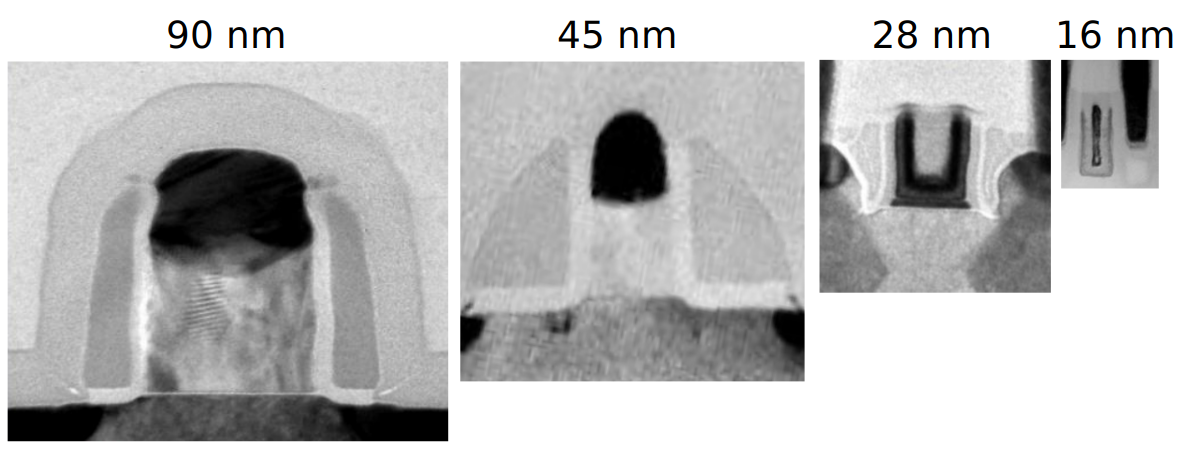
\includegraphics[width=\textwidth]{src/1/figures/technology_evolution.pdf}
  \caption{Recent evolution of NXP's automotive technology nodes \cite{evolution_technologies}}
  \label{fig:nxp-techno-increase}
\end{figure}

% Side effects of size reduction
As a side effect, integrated circuits become more fragile and sensitive.
Maximum tolerated voltage and current levels are smaller.
Above those limits, devices are degraded or destroyed.
The silicon area required for protecting the devices becomes a larger fraction of the complete chip area \cite{evolution_technologies}, and thus of the cost.

% Another trend in automotive - more electronic functions
Nowadays, new major features are developped in the automotive field.
The development of assisted or fully autonomous driving is seeing tremendous progress.
Autonomous vehicles take decisions and perform critical actions such as braking or steering the wheel.
Thoses features are implemented for safety purposes and put very high responsabilities on electronic modules.
Electric cars raise new challenges for safety as well, such as battery management.
Those features require more computing power, more sensing capabilities and more data to exchange.
As a consequence, the amount of \gls{ecu}s and electronic modules in a car is growing quickly.
Communication buses like the \gls{can} \cite{CAN} or \gls{lin} \cite{LIN} are shared by multiple systems and new standards appear for supporting higher bandwidths.
The CAN bus with Flexible Data rate (CAN-FD) is an example of this trend.

% Another trend is reduced power consumptions
Electrical power consumption has largely increased in vehicles.
Solutions are progressively set up to reduce it.
At the integrated circuit level, the main solution so far is to lower supply voltages.
With the most recent technology nodes, it is now common to find supply voltages near 1V.
Noise margins become very small, resulting in circuits far more sensitive to electrical disturbances.

% Harsh environment in the automotive field
The automotive field is also an harsh environment for electronic devices.
Equipements are exposed to a wide range of stresses.
A running engine generates plenty of vibrations and mechanical stress.
A lot of heat and thermal cycling is produced when the engine is on, and a vehicle is exposed to large temperature variations during its lifetime.
Electrical contacts, solder joints and connections suffer from these stresses, and must be designed to withstand them.
Electronic system are also exposed to a wide range of electrical stresses especially in the automotive field.
There are many sources of electrical stresses in a vehicle.
Transient disturbances can be generated natural phenomena, by the vehicle itself or some of its components.
When the engine is turned on for instance, the battery voltage can drop very low because of the amount of current drawn by the ignition.
This voltage drop can affect electronic systems and damage them.
This kind of disturbance is generated by the vehicle itself, but there is another major source of electrical stress coming from a natural phenomenon, called \gls{esd}.

% What is an ESD
An electrostatic discharge is the sudden flow of electricity between two objects of different charge.
It is the result of a local accumulation of electrostatic potential.
When a large enough potential difference is reached, a very rapid and violent discharge occurs.
It is common to record amplitudes in the range of thousands of volts and tens of amperes.
A study by Renault car manufacturer \cite{Renault-esd} estimates that electronic devices are exposed 10000 times to \gls{esd}s during their lifetime.
It has always been considered a very serious threat for electronic systems.

% Architecture systemes automobiles
In terms of architecture, a vehicle is constituted by a multitude of electronic modules, interconnected with cables.
This architecture raises some challenges for guaranting robustness against electrical disturbances.
A car is connected to the earth's ground through the tires, which is equivalent to a thick layer of insulating material.
Interconnected electronic systems need to share a good ground reference for them to communicate and work properly.
This function is assumed by the car's metallic body.
In \gls{dc} and at low frequencies, this reference is quite good because the vehicle's body is a very large chunck of metal with a very low resistance.
Electrostatic discharges are high frequency events, with significant frequency content up to a gigahertz.
In this frequency range, the car's body is not a low value resistor anymore and cables behave as large inductances.
As a result, electronic modules do not share a good reference and can be disturbed and fail to function properly.
For electrostatic discharges and \gls{emc} in general, cables are an important issue.
Inside a car, cables are not shielded and make great antennas that can both receive and emit radiated interferences.
Couplings between cables propagate interferences between interconnect domains.
Overall, the architecture of a vehicle is complex and sensitive to electrical disturbances.

\begin{figure}[!h]
  \centering
  \includegraphics[width=0.7\textwidth]{src/1/figures/systemintegration_01_uv-data.jpg}
  \caption{Architecture of electronic systems in a vehicle \cite{car-architecture}}
  \label{fig:car-architecture}
\end{figure}

% Fiabilite vis a vis des ESD
In summary, the amount of electronic devices is increasing and in the same time they become more sensitive.
Systems are complex to study and analyse, have more responsabilities in regards of our safety, and the surrounding environment is very harsh.
Studying and predicting all kinds of failures is important in order to avoid them early.
In the \gls{esd} field, there are two kinds of failures to consider.
The hardware failure, or hard-failure, is when an electronic device is permanently damaged.
There can be multiple signatures, such as apparition of minor defects, important variation of intrisic properties or complete destruction (see Fig. \ref{fig:esd-failures}).
Semiconductor devices are particularly sensitive to electrostatic discharges \cite{impactESDsemiconductors} and require specific protection.
Recently, a new class of failures is being studied, motivated by new requirements for operating safety.
Soft-failure, or functional failure, is when an electronic device fails temporarily to perform its function, because of an electrical disturbance.
In this scenario, different levels of severity can be identified depending on the impact of the failure on the rest of the system.
In the best case, a module is momentarily disturbed by a discharge but recovers immediately without noticeable impact.
In a more severe scenario, some minor functionnalities such as entertainment systems are frozen, requiring an user intervention to recover, in the form of restarting the vehicle for instance.
The same kind of issue with airbags or assisted braking would be considered a lot more severe, because user safety can no longer be guaranteed.
Functionnal failures raise new kind of challenges for the analysis, and in particular with the scale factor.
A functionnal failure may happen because a few transistors inside a chip were disturbed, but the consequences can be visible much higher in the hierarchy and at the scale of an entire vehicle.
In regard of those challenges, new analysis and predictions methods are required against soft-failures caused by electrostatic discharges.

\begin{figure}[!h]
  \centering
  
\includegraphics[width=\textwidth]{src/1/figures/esd_failures.pdf}
  \caption{Different kinds of ESD-induced failures}
  \label{fig:esd-failures}
\end{figure}

%TODO: Explain the cost of fixing an issue early vs lately ?

% Comment predire ces defaillances fonctionnelles
First research on the topic was published by F. Caignet and N. Lacrampe in 2007 \cite{}.
After a few years, the industry widely acknowledged the problem, reinforced by the current automotive trends.
A large amount of research at the system level was published in EOS/ESD symposia 2012 \cite{} and 2013 \cite{}.
The draft standard IEC 62433-6 aims to provide a base framework for soft-failures analysis and prediction.
So far, the litterature is focused on system-level analysis.
There is currently no real work at the component level or studies performed inside the design of an integrated circuit.
This PhD explored the topic and tries to provide some new leads for future research.

% Conception methods
Beyond studying failures inside integrated circuits, it is important to keep in mind how chips are designed and developped.
This is important to propose solutions that are actually implementable.
This entire process from the specification to the manufacturing of a product is called the design flow.
During this process, there are many teams and people involved.
Modeling team creates electrical model of technology components.
Design team assembles component together to create integrated functions that conform to the specification.
Layout team translates the symbolic view of electrical netlists into the series of masks and layers required by manufacturing.
The laboratory tests manufactured parts and runs investigations in case of failures.
The \gls{esd} and \gls{emc} team has the particularity to interact will all teams because issues and solutions can be found in any step of the design flow.
Overall, the integrated circuits are designed hierarchically and the flow is a bottom-up process.
Fundamental bricks are assembled together in rising complexity to create the required functions.
The main source of delay in this process is the long delay for the feedback due to the manufacturing.
Designs are put on silicon but the parts are tested only after manufacturing, which can occur several months later.
To gain time to market and be competitive, it is essential to reduce to a bare minimum the amount of design-manufacturing-testing cycles.
This is why any simulation tool able to predict early any kind of failure (and functionnal failures among them) is very valuable for silicon design companies.

\begin{figure}[!h]
  \centering
  
\includegraphics[width=\textwidth]{src/1/figures/overview_flow.pdf}
  \caption{Highly simplified integrated circuit design flow - specification, symbolic view, layout, silicon}
  \label{fig:ic-design-flow}
\end{figure}

% Presentation des chapitres
%
Chapter \ref{chap:1} details how electrostatic discharge physically appear, how to reproduce them in laboratory conditions and summarizes recent litterature.
This preliminary work highlights how functional failures appear and how they impact electronic devices.
It is demonstrated that so far integrated circuits are studied as black-box electrical objects.
Stresses are injected on external inputs while external outputs are monitored for failures.
The amount of silicon-level studies and research remains small.

%
Chapter \ref{chap:2} presents a modeling method for simulating \gls{esd} waveforms up to the integrated circuit inputs.
The first challenge for understanding soft-failures at silicon-level is to determine what fraction of an incoming \gls{esd} actually reaches the integrated circuit.
Between the injection point of a stress and the disturbed circuit, many devices are be connected such as cables, discrete devices, etc.
Each element interacts with the discharge, absorbs a part of its current or changes the waveform.
A model library of common electrical elements found in \gls{esd} testing environment has been constructed and is detailed.

%
A case of soft-failure in an integrated circuit is explained in chapter \ref{chap:3}.
In a first phase, measurement data is obtained at the board level and the failure is explained.
Simulations are run to understand how failures appear, and more specifically how a short electrical event can disturb an integrated circuit for a long period of time.
In a second phase, the integrated function is placed onto a custom testchip.
Specific on-silicon structures were designed to gather measurement data on electrical nets that are not physically accessible.
All these measurements are performed for the purpose of estimating the accuracy of integrated circuit \gls{esd} simulations.
There are two main potential sources of error that are checked.
Silicon technology device models are not designed to function for extremely fast transient transient disturbances.
Also, standard simulations do not take parasitic devices into account, such as metal track resistances and parasitic couplings.
Measurement data is confronted to simulations in order to verify the validity of models.
Analysis of the failure led to the development of a testchip, to put on silicon the same failing function but with a more convenient environment for measurements and investigation.

%
When issues are discovered late in the testing lab, analysis is performed manually, by trial and error, searching inside the design why the function is failing.
It is a complex and time-consuming process.
The core research of this work focuses proposing new analysis methods and tools for electrical simulations.
It is detailled in chapter \ref{sec:methods-operating-esd-analysis}.

%
Finally, a new test generator was developed to overcome some issues found when debugging silicon-level failures caused by system level \gls{esd} testers.
The principle of operation and architecture of the generator is described in chapter \ref{sec:tlp-hmm}.
The conclusion summarizes the work achieved during the PhD, highlights the most notable discoveries, and identifies follow-up work and research topics that could be worth pursuing.
Some part of the research work also focused towards \gls{esd} testers.
System-level \gls{esd} guns \cite{iec61000-4-2, iso10605} constitute a major testing and qualification tool, but bring too much complexity during silicon-level investigation.
To overcome this issue, a new stress generator based on a \gls{tlp} is proposed in chapter \ref{sec:tlp-hmm}.
It produces the same compliant waveform than those standards, but with some interesting advantages.
It is not a drop-in replacement but can be interesting as an investigation tool.

%
Final conclusions and potential following work are detailed in chapter \ref{sec:final-conclusion}.
